\documentclass[aspectratio=169,10pt]{beamer}
\newcommand{\reporoot}{../..}
% Shared preamble of the main deck and the topic decks.
% Define \reporoot (the path from the .tex file to the repository root)
% before \input-ing this file.
\usetheme[progressbar=frametitle,numbering=fraction,sectionpage=progressbar]{metropolis}

\usepackage{amsmath,amssymb}
\usepackage{booktabs}
\usepackage{graphicx}
\usepackage{tikz}
\usetikzlibrary{arrows.meta,positioning,decorations.pathreplacing}
\usepackage[authoryear,round]{natbib}
\usepackage{xcolor}

\graphicspath{{\reporoot/figures/}}

% Every number on the slides is produced by experiments/*.py and read from here.
\input{\reporoot/results/e1_markov_book.tex}
\input{\reporoot/results/e2_best_queues.tex}
\input{\reporoot/results/e3_queue_reactive.tex}
\input{\reporoot/results/e4_hawkes.tex}
\input{\reporoot/results/e5_signature.tex}
\input{\reporoot/results/e6_propagator.tex}
\input{\reporoot/results/e7_market_making.tex}
\input{\reporoot/results/e8_ofi.tex}
\input{\reporoot/results/e9_queue_value.tex}
\input{\reporoot/results/e10_markouts.tex}
\input{\reporoot/results/e11_glft_exact.tex}
\input{\reporoot/results/e12_signal.tex}
\input{\reporoot/results/e13_lvr.tex}
\input{\reporoot/results/e14_mlofi.tex}
\input{\reporoot/results/e15_rate_estimation.tex}
\input{\reporoot/results/e16_queue_reactive_price.tex}
\input{\reporoot/results/e17_hawkes_pitfalls.tex}
\input{\reporoot/results/e18_propagator_estimation.tex}
\input{\reporoot/results/e19_latent_book.tex}
\input{\reporoot/results/e20_microprice.tex}
\input{\reporoot/results/e21_fill_estimation.tex}
\input{\reporoot/results/e22_glosten_milgrom.tex}
\input{\reporoot/results/e23_cdl_on_book.tex}

\newcommand{\E}{\mathbb{E}}
\newcommand{\Var}{\operatorname{Var}}
\newcommand{\OFI}{\mathrm{OFI}}
\newcommand{\dd}{\mathrm{d}}
\newcommand{\src}[1]{\par\vfill{\scriptsize\color{gray}#1}}
\definecolor{accent}{HTML}{0C5DA5}
\definecolor{warn}{HTML}{C0392B}
\newcommand{\hl}[1]{\textcolor{accent}{\textbf{#1}}}

\setbeamerfont{footnote}{size=\tiny}
\setbeamerfont{caption}{size=\scriptsize}

\author{Yaohui Shu}
\institute{Stony Brook University}
\date{October 2026}

% Topic decks: a references frame that lists only the works cited in the deck.
\newcommand{\deckreferences}{%
  \begin{frame}[allowframebreaks]{References}
    \tiny
    \renewcommand{\bibsection}{}
    \bibliographystyle{plainnat}
    \bibliography{\reporoot/slides/refs}
  \end{frame}}

% Topic decks: the standard "where this fits" footer on the title frame.
\newcommand{\deckseries}{Deep dive in the series \emph{Stochastic Models of the Limit Order Book}}

% Topic decks: \decknumber{n} puts the series line under the date on the title page.
\newcommand{\decknumber}[1]{\institute{Stony Brook University\hfill{\scriptsize\color{gray}Deep dive #1 of 9}}}


\title{The Best Queues}
\subtitle{Cont-de Larrard: direction, timing and volatility from two queues}
\decknumber{2}

\begin{document}

\maketitle

\begin{frame}{The question}
  \small
  \begin{columns}[T]
    \begin{column}{0.55\textwidth}
      In a liquid large-tick stock almost all activity happens at the best bid and ask. \hl{Can two queues explain the next price move, its timing, and volatility?}
      \begin{itemize}
        \item The direction of the next move is what a quote should anticipate.
        \item The time to the next move sets how long a quote is exposed.
        \item The volatility formula links microstructure (rates, depth) to the risk an LP carries over minutes.
      \end{itemize}
    \end{column}
    \begin{column}{0.42\textwidth}
      \begin{alertblock}{In this deck}
        \small
        \begin{enumerate}
          \item First passage of a queue to zero.
          \item $p_\uparrow$, durations, diffusion limit.
          \item Fitting it to a richer book, and the statistics of conditional frequencies.
          \item Evidence from \citet{cont2013price}.
        \end{enumerate}
      \end{alertblock}
    \end{column}
  \end{columns}
\end{frame}

\begin{frame}{The model}
  \small
  One-tick spread. The bid queue $q_b$ and ask queue $q_a$ (orders) each move independently:
  \[ q \to q + 1 \text{ at rate } \lambda, \qquad q \to q - 1 \text{ at rate } \nu = \mu + \theta, \]
  with $\lambda$ the limit order rate per queue, $\mu$ the market order rate and $\theta$ the cancellation rate, all in s$^{-1}$ and \emph{constant} (not per order).
  \begin{itemize}
    \item When the ask empties the price moves up one tick $\delta$; when the bid empties it moves down.
    \item After a move both queues are redrawn from a distribution $f$ on $\mathbb{N}^2$; this ``regeneration'' is what makes the price a random walk.
  \end{itemize}
  \vspace{0.3em}
  \centering
  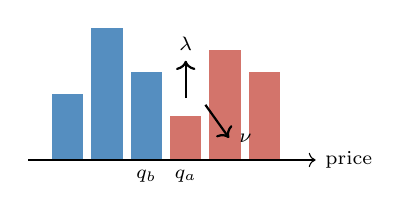
\begin{tikzpicture}[x=0.5cm,y=0.28cm]
    \foreach \h [count=\i] in {4,6,3} {\fill[accent!70] ({-\i+0.1},0) rectangle ({-\i+0.9},\h);}
    \foreach \h [count=\i] in {2,5,4} {\fill[warn!70] ({\i-0.9},0) rectangle ({\i-0.1},\h);}
    \draw[->] (-3.5,0) -- (3.8,0) node[right] {\scriptsize price};
    \node[below] at (-0.5,0) {\scriptsize $q_b$};
    \node[below] at (0.5,0) {\scriptsize $q_a$};
    \draw[->,thick] (0.5,2.8) -- (0.5,4.5) node[above] {\scriptsize $\lambda$};
    \draw[->,thick] (1.0,2.5) -- (1.6,1.0) node[right] {\scriptsize $\nu$};
  \end{tikzpicture}
\end{frame}

\begin{frame}{First passage and the next move}
  \small
  \begin{columns}[T]
    \begin{column}{0.52\textwidth}
      A queue of size $q$ is a birth-death walk; its time $\tau_q$ (s) to hit zero has density
      \[ f_q(t) = \frac{q}{t}\Big(\frac{\nu}{\lambda}\Big)^{q/2} I_q\big(2\sqrt{\lambda\nu}\,t\big)\,e^{-(\lambda+\nu)t}, \]
      with $I_q$ the modified Bessel function of the first kind. The queues are independent, so
      \[ p_\uparrow(q_b,q_a) = \int_0^\infty f_{q_a}(t)\,P(\tau_{q_b} > t)\,\dd t, \]
      \[ P(\tau > t \mid q_b, q_a) = P(\tau_{q_b} > t)\,P(\tau_{q_a} > t). \]
    \end{column}
    \begin{column}{0.45\textwidth}
      \textbf{Balanced case} $\lambda = \nu$, large queues: $(q_b, q_a)$ is close to a planar Brownian motion stopped on the axes, and
      \[ p_\uparrow \approx \tfrac{2}{\pi}\arctan(q_b/q_a). \]
      \textbf{Heavy tail.} $P(\tau > t) \approx q_b q_a/(\pi\lambda t)$: the mean time between moves is infinite.

      \vspace{0.3em}
      \textbf{Unbalanced} $\lambda < \nu$: queues drain on average, $\E[\tau_q] = q/(\nu - \lambda)$, and durations have a light tail.
    \end{column}
  \end{columns}
\end{frame}

\begin{frame}{Volatility from order flow}
  \small
  Balanced case. Let $M_F = \sum_{x,y} x\,y\,f(x,y)$ (orders$^2$) be the mean product of queue sizes after a move. Because $P(\tau > t) \sim M_F/(\pi\lambda t)$, the truncated mean duration grows like $(M_F/\pi\lambda)\ln(\lambda t)$, and the number of moves by time $t$ like $\pi\lambda t/(M_F \ln(\lambda t))$. Each move is $\pm\delta$, so for independent moves over a horizon $T$ (s)
  \[ \Var(S_T - S_0) \approx \frac{\pi\lambda\,\delta^2}{M_F}\,\frac{T}{\ln(\lambda T)} \quad\Longrightarrow\quad \sigma^2 \propto \frac{\lambda\,\delta^2}{M_F}. \]
  \begin{itemize}
    \item \citet{cont2013price} prove the diffusion limit on the time scale $t\,n\ln n$.
    \item Reading: more limit order flow raises volatility; deeper queues after a move lower it.
    \item If increments are negatively correlated (bid queue usually smaller than the new ask queue after an up move), the walk mean-reverts at short lags.
  \end{itemize}
  \vspace{0.2em}
  Not checked numerically here: the $\ln T$ correction makes the diffusion limit slow to reach in simulation.
\end{frame}

\begin{frame}{Closed forms against simulation}
  \centering
  \includegraphics[width=0.88\textwidth]{fig2_best_queues.png}
  \small
  \begin{itemize}
    \item Monte Carlo ($\EtwoNmc$ paths per point) matches the closed form within $\EtwoMaxDev$ standard errors; an exact sparse linear solve agrees to $2\times10^{-3}$.
    \item The duration tail $q_bq_a/(\pi\lambda t)$ is within $\EtwoTailErr\%$ of the exact survival at $10^4$ s. The arctangent law is off by $\EtwoArctanErrSmall$ at $(2,5)$.
  \end{itemize}
\end{frame}

\begin{frame}{Statistics: fitting the model, and samples that are not independent}
  \small
  \begin{columns}[T]
    \begin{column}{0.5\textwidth}
      \textbf{Fitting.} From one-tick-spread periods of total length $T_1$ (s):
      \[ \hat\lambda = \frac{\#\{\text{orders joining a best queue}\}}{2T_1}, \]
      \[ \hat\nu = \frac{\#\{\text{market orders + cancels at the best}\}}{2T_1}. \]
      Then $\hat p_\uparrow(q_b, q_a)$ from the closed form.

      \vspace{0.3em}
      \textbf{Testing.} Compare with the empirical frequency of up moves given $(q_b, q_a)$.
    \end{column}
    \begin{column}{0.46\textwidth}
      \textbf{The trap.} If every book event is a sample, all samples between two price moves share one outcome. In the simulated book, state $(2,5)$ has thousands of samples but only about a minute of exposure.

      \vspace{0.3em}
      Binomial errors $\sqrt{p(1-p)/n}$ are then far too small. Treat all samples before the same move as one \hl{cluster}:
      \[ \widehat{\Var}(\hat p) = \frac{1}{n^2}\sum_{c}\Big(\sum_{i\in c}(y_i - \hat p)\Big)^2 , \]
      with $y_i \in \{0,1\}$ the outcome of sample $i$.
    \end{column}
  \end{columns}
\end{frame}

\begin{frame}{Fitting constant rates to a book whose rates are not constant}
  \centering
  \includegraphics[width=0.84\textwidth]{fig23_cdl_on_book.png}
  \begin{columns}[T]
    \begin{column}{0.5\textwidth}
      \footnotesize
      Power-law Markovian book (deck 1), $\EtwentythreeNevents$ events, $\EtwentythreeMoves$ mid moves. In it the best queues shrink at $\mu + \theta q$, which grows with $q$. Fitted CdL rates: $\hat\lambda = \EtwentythreeLam$, $\hat\nu = \EtwentythreeNu$ s$^{-1}$.
    \end{column}
    \begin{column}{0.46\textwidth}
      \footnotesize
      Over $\EtwentythreeCells$ cells, CdL is off by $\EtwentythreeMaeCdl$ on average (worst $\EtwentythreeMaxErrCdl$); the exact answer for state-dependent rates is off by $\EtwentythreeMaeExact$, within $\EtwentythreeMaxZExact$ clustered s.e. CdL overstates how decisive imbalance is: with $\nu$ constant, long queues drain too slowly.
    \end{column}
  \end{columns}
\end{frame}

\begin{frame}{What the data show}
  \small
  \citet{cont2013price}, NYSE stocks on 26 June 2008:
  \begin{itemize}
    \item \textbf{One-tick spread most of the time}: 98.82\% of observations for Citigroup, 98.80\% for General Electric, 98.71\% for General Motors.
    \item \textbf{Nearly balanced flow}: the estimated limit order rate is slightly below the rate of market orders plus cancellations, with a small gap.
    \item \textbf{Asymmetric regeneration}: after an up move the new bid queue is usually smaller than the new ask queue (for Citigroup the relevant probability exceeds 0.7), so price increments are negatively correlated at high frequency.
    \item \textbf{Volatility across stocks}: for Dow Jones stocks the standard deviation of 10-minute price changes rises roughly in proportion to the rate-over-depth ratio predicted by the model.
    \item Conditional probabilities of an up move given the queues agree well with Citigroup tick data.
  \end{itemize}
  \vspace{0.2em}
  The arctangent shape is also the basis of the \hl{micro-price} \citep{stoikov2018micro}, deck 6.
\end{frame}

\begin{frame}{Discussion}
  \small
  \begin{columns}[T]
    \begin{column}{0.5\textwidth}
      \textbf{What it gets right}
      \begin{itemize}
        \item Imbalance predicts direction, with a closed form.
        \item Heavy-tailed durations: long quiet spells between moves.
        \item A volatility formula with no price data in it.
      \end{itemize}
      \textbf{What it leaves out}
      \begin{itemize}
        \item Depletion that depends on queue size (fixed by the exact state-dependent solve here, or by queue-reactive models, deck 3).
        \item Memory and clustering of events (deck 4).
        \item Spreads wider than one tick, so small-tick assets are out of scope.
      \end{itemize}
    \end{column}
    \begin{column}{0.46\textwidth}
      \textbf{For a liquidity provider}
      \begin{itemize}
        \item $p_\uparrow$ is the probability that a resting bid becomes stale; use the state-dependent version when cancellation scales with queue size.
        \item The duration law sets how long a quote sits exposed; a $1/t$ tail means occasional very long exposures.
        \item Conditional frequencies from tick data need clustered errors, or every cell looks significant.
      \end{itemize}
      \textbf{Open question.} A tractable version with history (Hawkes) and state dependence that keeps closed forms for $p_\uparrow$.
    \end{column}
  \end{columns}
\end{frame}

\begin{frame}[fragile]{Reproduce}
  \small
  Code: \texttt{best\_queues.py} (closed forms, simulation), \texttt{queue\_position.p\_up\_state\_dependent} (exact solve for $\mu + \theta q$), \texttt{markov\_lob.empirical\_p\_up} (frequencies with clustered errors). Experiments: \texttt{e2\_best\_queues.py}, \texttt{e23\_cdl\_on\_book.py}.
\begin{verbatim}
from stochastic_lob import best_queues as bq
bq.p_up(q_b=2, q_a=5, lam=1.0, nu=1.2)      # P(next move is up)
bq.duration_survival(t=60.0, q_b=2, q_a=5, lam=1.0, nu=1.0)
\end{verbatim}
\end{frame}

\deckreferences
\end{document}
